\documentclass[12pt]{article}

\usepackage[utf8]{inputenc}
\usepackage[T1]{fontenc}
\usepackage[spanish]{babel}
\usepackage{graphicx}
\usepackage{listings}
\usepackage{caption}
\usepackage{subcaption}
\usepackage[right=2cm,left=2cm,top=2cm,bottom=2cm]{geometry}
\usepackage{hyperref}
\usepackage{fancyhdr}
\usepackage{color}
\usepackage[export]{adjustbox}
\usepackage{graphicx}
\usepackage{float}
\usepackage{changepage}
\usepackage{multicol}
\usepackage{imakeidx}
\usepackage[spanish]{babel}
\usepackage[backend=biber]{biblatex}

\pagestyle{fancy}
\renewcommand{\footrulewidth}{0.4pt}
\setlength{\headheight}{15pt}


\fancyhead[L]{ CEIABD – MIA }
\fancyhead[R]{ Páez Anguita, Víctor }
\fancyfoot[L]{IES Gran Capitán}


\begin{document}

\begin{titlepage}
    \begin{center}
      \Large \bfseries{}
    \end{center}
    \vspace{0.1cm}
    \begin{center}
      \Large \bfseries{}
    \end{center}
    \vspace{0.1cm}
    \begin{center}
     \Large \bfseries{Aplicación de la IA en diferentes campos}
    \end{center}
    \vspace{0.0001cm}
    \begin{center}
        Departamento de informática \\ I.E.S. Gran Capitán - Córdoba
    \end{center}
        \vspace{2 cm}
\begin{figure}[h!]
    \centering
    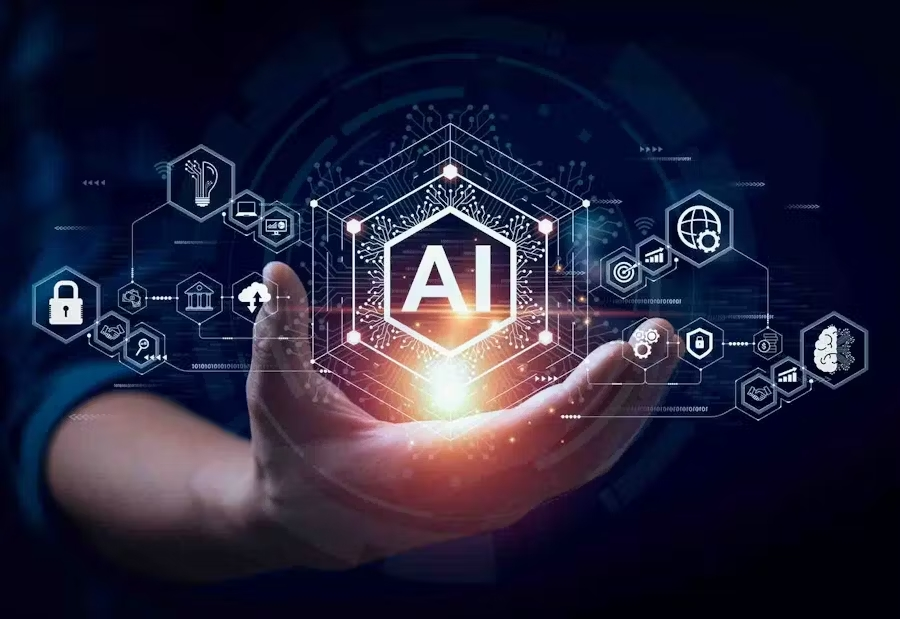
\includegraphics[width=.6\textwidth]{ramas_ia_1.jpg}
    \label{fig:my_label}
\end{figure}
    \vspace{0.2 cm}
    \begin{center}
        Inteligencia artificial y Big data \\ Córdoba, 5 de Noviembre 2024
    \end{center}
    \vspace{4 cm}
\null\hfill \textbf{Desarrollado por:}
\\
\\
\null\hfill José Luis Hidalgo
\\
\null\hfill Marta Lopez
\\
\null\hfill Víctor Páez Anguita
\clearpage
\end{titlepage}

%%%%%%%%%%%%%%%%%%%%%%%%%%%Index%%%%%%%%%%%%%%%%%%%%%%%%%%%%%%%%
\tableofcontents
\clearpage
%%%%%%%%%%%%%%%%%%%%%%%%%%%Index%%%%%%%%%%%%%%%%%%%%%%%%%%%%%%%%

\section{Introducción}

En este documento veremos los distintos usos que se le da a la Inteligencia artificial en diferentes areas
de trabajo. Además, se explicarán los beneficios que aportan a sus respectivos campos y tambíen sus desventajas.

\section{Agricultura}
\section{Banca}
\section{Ciberseguridad}
\section{Atención sanitaria}
\section{Logística: rutas y optimización}
\section{Telecomunicaciones: optimización de redes}
\subsection{Descripción general}
La optimización de redes en telecomunicaciones busca mejorar el rendimiento, la eficiencia y la capacidad de las redes para 
satisfacer la creciente demanda de conectividad rápida y estable. Con el aumento de dispositivos conectados y el tráfico de datos, 
es esencial optimizar las redes para evitar sobrecargas y mantener una alta calidad de servicio.
\subsection{Como funcionan}
\begin{itemize}
    \item Inteligencia Artificial (IA) y Machine Learning (ML):
    \begin{itemize}
        \item La IA y el ML permiten analizar grandes volúmenes de datos en tiempo real para optimizar el rendimiento de la red. Estas tecnologías 
        pueden predecir posibles fallos y ajustar los recursos de red en función de la demanda.
        \item Predicción de fallas: Algoritmos de ML identifican patrones que anticipan problemas en la red, lo cual permite realizar mantenimiento 
        preventivo.
        \item Automatización: La IA ajusta automáticamente parámetros de la red, como el ancho de banda, en función del tráfico actual, 
        minimizando la congestión. 
    \end{itemize}

    \item Gestión de la Calidad de Servicio (QoS):
    \begin{itemize}
        \item La QoS garantiza que aplicaciones críticas, como llamadas de voz o videoconferencias, tengan prioridad sobre aquellas menos 
        sensibles a la latencia, optimizando así la experiencia del usuario.
        \item Priorización de tráfico: Se asigna ancho de banda preferente a servicios que requieren baja latencia y se limitan aquellos de
        menor importancia en tiempo real. 
    \end{itemize}

    Control de congestión: Mediante algoritmos que monitorizan el tráfico, la red se ajusta en tiempo real para evitar sobrecargas.
    \item Optimización del Uso del Espectro en Redes Inalámbricas:
    \begin{itemize}
        \item El espectro es un recurso limitado en telecomunicaciones, y optimizar su uso es esencial para maximizar la capacidad de la red 
        sin afectar la calidad de la conexión.
        \item MIMO (Multiple Input Multiple Output): Aprovecha múltiples antenas para reducir la interferencia y mejorar la capacidad de la red.
        \item Celdas pequeñas y femtoceldas: Estas soluciones ayudan a cubrir áreas de alta demanda mediante el uso de celdas de menor alcance, 
        lo que reduce la carga en la red principal y mejora la cobertura.
        \item Agrupamiento de portadoras: Utilizado en tecnologías 4G y 5G, combina diferentes bandas de frecuencia para mejorar la velocidad 
        y estabilidad de la conexión.
    \end{itemize}

    \item Optimización de Redes de Acceso y Núcleo:
    \begin{itemize}
        \item Las redes de acceso y núcleo (core) conectan dispositivos con la infraestructura central de la red y son fundamentales para la 
        eficiencia y confiabilidad general.
        \item Redes Definidas por Software (SDN): Permiten una gestión centralizada de los flujos de datos mediante software, lo cual 
        optimiza el uso de recursos y permite configuraciones flexibles.
        \item Virtualización de Funciones de Red (NFV): Reemplaza equipos físicos por software, lo cual reduce costos y permite escalar 
        los recursos de manera más eficiente.
    \end{itemize}

\end{itemize}

\begin{figure}[h!]
    \centering
    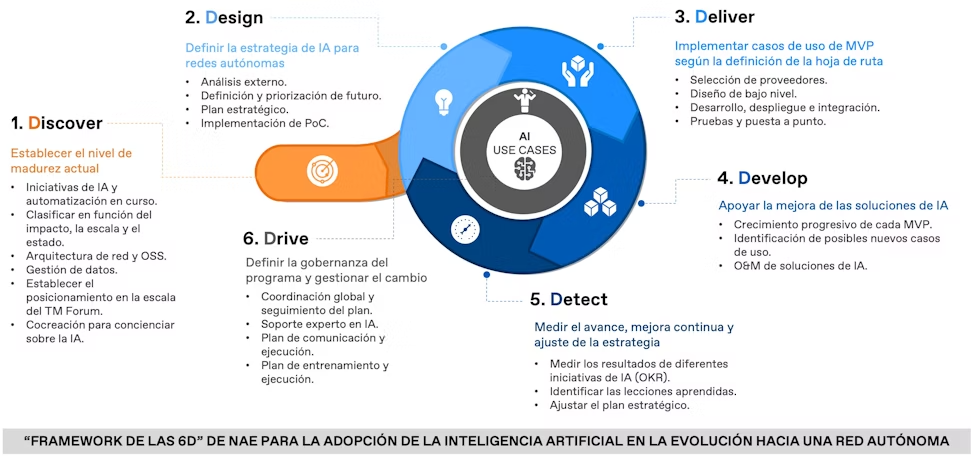
\includegraphics[width=.6\textwidth]{teleco.png}
    \label{fig:my_label}
\end{figure}

\subsection{ventajas}
\begin{itemize}
    \item Mejora en la calidad del servicio: 
    Reduce la latencia y mejora la estabilidad en servicios como videollamadas y juegos en línea.
    \item Uso eficiente de recursos: 
    Optimiza el uso del espectro y reduce los costos operativos mediante la virtualización y el SDN.
    \item Mantenimiento predictivo: 
    Evita fallas en la red, minimizando el tiempo de inactividad y aumentando la disponibilidad.
\end{itemize}

\subsection{Desventajas}
\begin{itemize}
    \item Costos de implementación: 
    Integrar IA, ML y virtualización requiere una inversión inicial significativa.
    \item Dependencia de la tecnología: 
    La automatización y el control centralizado pueden ser vulnerables a fallos en los sistemas de software.
    \item Riesgos de seguridad: 
    La optimización y virtualización aumentan los puntos de vulnerabilidad en la red, lo cual exige medidas de ciberseguridad adicionales.
\end{itemize}

\section{Juegos: creación de agentes inteligentes}
\subsection{Descripción general}
Los agentes inteligentes en videojuegos son sistemas de IA diseñados para simular el comportamiento humano o para actuar de manera
autónoma en función de un entorno o de las acciones del jugador. Estos agentes mejoran la jugabilidad y la experiencia al reaccionar 
de manera dinámica e imitar la toma de decisiones humanas.
\subsection{Como funcionan}
\begin{itemize}
    \item Modelos basados en reglas:
    Este es el enfoque más sencillo, donde los personajes o agentes actúan según un conjunto de reglas preestablecidas. 
    Estos modelos tienen limitaciones, ya que no se adaptan a nuevas situaciones.
    \item Aprendizaje por refuerzo: 
    Utilizado especialmente en juegos que requieren agentes adaptativos. 
    En este enfoque, el agente toma decisiones basadas en recompensas o penalizaciones, mejorando su comportamiento a 
    medida que aprende cuáles acciones son óptimas. Un ejemplo de esto es AlphaGo, el agente desarrollado por DeepMind, 
    que aprendió a jugar al juego de mesa Go, superando a jugadores humanos.
    \item Redes neuronales y algoritmos evolutivos: 
    Permiten que el agente aprenda de patrones complejos y ajuste su comportamiento en tiempo real, incluso sin reglas explícitas, 
    solo observando el entorno. Los algoritmos evolutivos pueden “cruzar” las características de los agentes exitosos, permitiendo a 
    los agentes evolucionar con el tiempo.
\end{itemize}

\begin{figure}[h!]
    \centering
    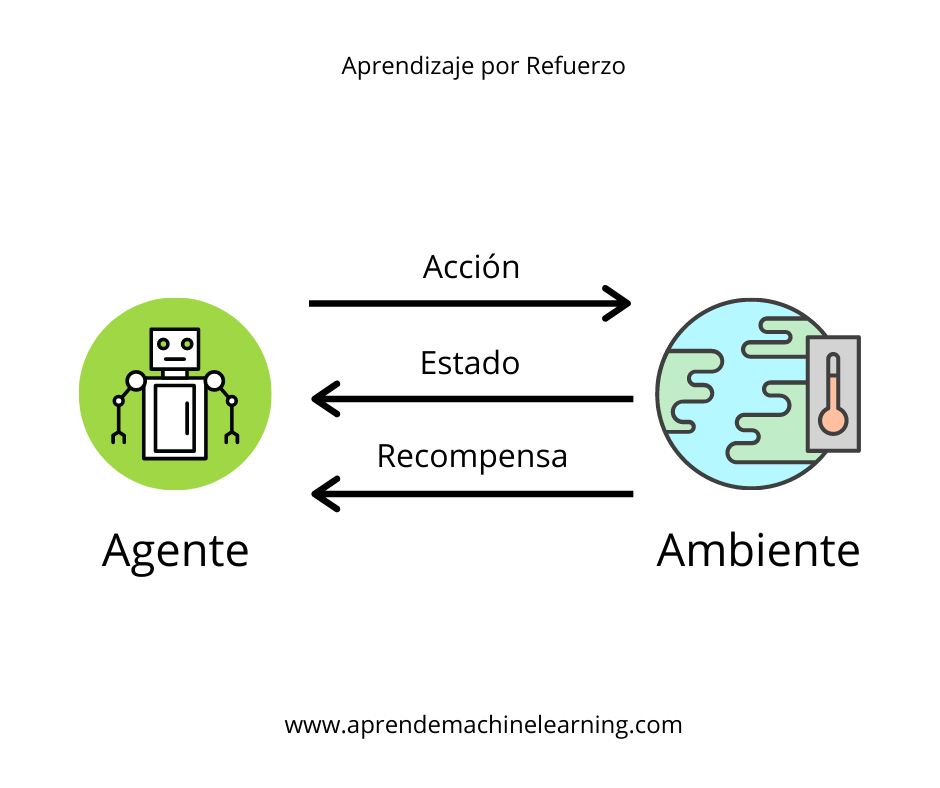
\includegraphics[width=.6\textwidth]{AprendizajeRefuerzo-global.png}
    \label{fig:my_label}
\end{figure}

\subsection{ventajas}
\begin{itemize}
    \item Los agentes pueden crear experiencias de juego desafiantes y adaptativas.
    \item Los jugadores pueden enfrentarse a oponentes de IA que evolucionan y se vuelven más sofisticados.
\end{itemize}

\subsection{Desventajas}
\begin{itemize}
    \item El comportamiento de la IA puede volverse impredecible o incluso frustrante si es demasiado difícil.
    \item El desarrollo y la optimización de agentes inteligentes requieren muchos recursos.
\end{itemize}

\section{Arte: Creatividad}
\subsection{Descripción general}

La inteligencia artificial en arte implica la generación de imágenes, estilos y composiciones visuales. Estas creaciones suelen 
combinarse con el trabajo humano o se generan por completo mediante IA, resultando en obras de arte que, en algunos casos, no son 
distinguibles de las creadas por humanos.

\subsection{Como funcionan}
\begin{itemize}
    \item Redes Generativas Antagónicas (GAN): 
    Las GAN constan de dos redes neuronales (generador y discriminador) que compiten entre sí. El generador intenta crear imágenes 
    convincentes mientras que el discriminador evalúa si son reales o artificiales, perfeccionando así la calidad de las imágenes generadas. 
    Este tipo de red es ideal para crear obras de arte nuevas y únicas.
    \item Transferencia de estilo neuronal: 
    En este proceso, un modelo de IA aplica el estilo de una obra de arte a otra imagen. 
    Esto se logra extrayendo y combinando patrones de color y forma, permitiendo que una fotografía, 
    por ejemplo, se asemeje al estilo de Van Gogh o Picasso.
    \item Procesamiento de imágenes:
    Modelos de visión artificial detectan patrones y crean nuevas composiciones basadas en elementos artísticos conocidos. 
    También permiten realizar modificaciones como ajustes de color y estilo, basándose en grandes bases de datos de imágenes.
\end{itemize}

\begin{figure}[h!]
    \centering
    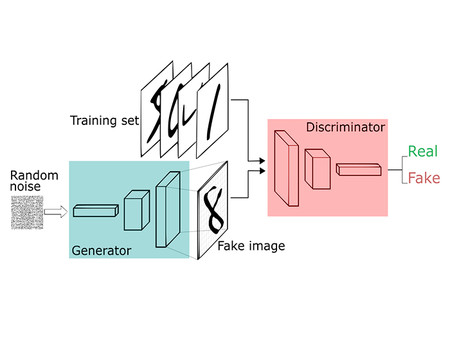
\includegraphics[width=.6\textwidth]{GAN.jpg}
    \label{fig:my_label}
\end{figure}

\subsection{ventajas}
\begin{itemize}
    \item Democratiza la creación de arte y permite a cualquier persona experimentar con el arte digital.
    \item Amplía las posibilidades creativas, ofreciendo nuevas formas de expresión artística y herramientas colaborativas.
\end{itemize}

\subsection{Desventajas}
\begin{itemize}
    \item Puede llevar a la desvalorización del trabajo artístico humano y a una posible dependencia de la IA para la creatividad.
    \item La IA podría imitar estilos sin consentimiento, generando riesgos de apropiación cultural.
\end{itemize}

\section{Escritura: corrección y generación de texto}
\subsection{Descripción general}
La IA en el ámbito de la escritura facilita la corrección automática, la generación de texto y la asistencia en redacción. 
Estos modelos permiten a los usuarios escribir con menos errores gramaticales, mejorar el estilo y generar contenido automáticamente 
en diferentes contextos.

\subsection{Como funcionan}
\begin{itemize}
    \item Modelos de lenguaje: 
    Los modelos de lenguaje actuales como GPT (Generative Pre-trained Transformer), BERT (Bidirectional Encoder Representations from Transformers)
    y T5 (Text-To-Text Transfer Transformer) se entrenan con grandes volúmenes de texto para predecir las palabras siguientes en una oración. 
    Estos modelos pueden generar texto coherente que se ajusta al contexto dado.
    \item Corrección gramatical:
    Utilizan modelos supervisados que identifican errores en el texto basándose en patrones de contexto. Estas herramientas son especialmente 
    útiles en software de edición de texto como Grammarly.
    \item Generación creativa de texto:
    Las IA como ChatGPT generan contenidos narrativos, académicos o incluso publicitarios, ajustándose al tono, estilo y longitud deseados.
\end{itemize}

\begin{figure}[h!]
    \centering
    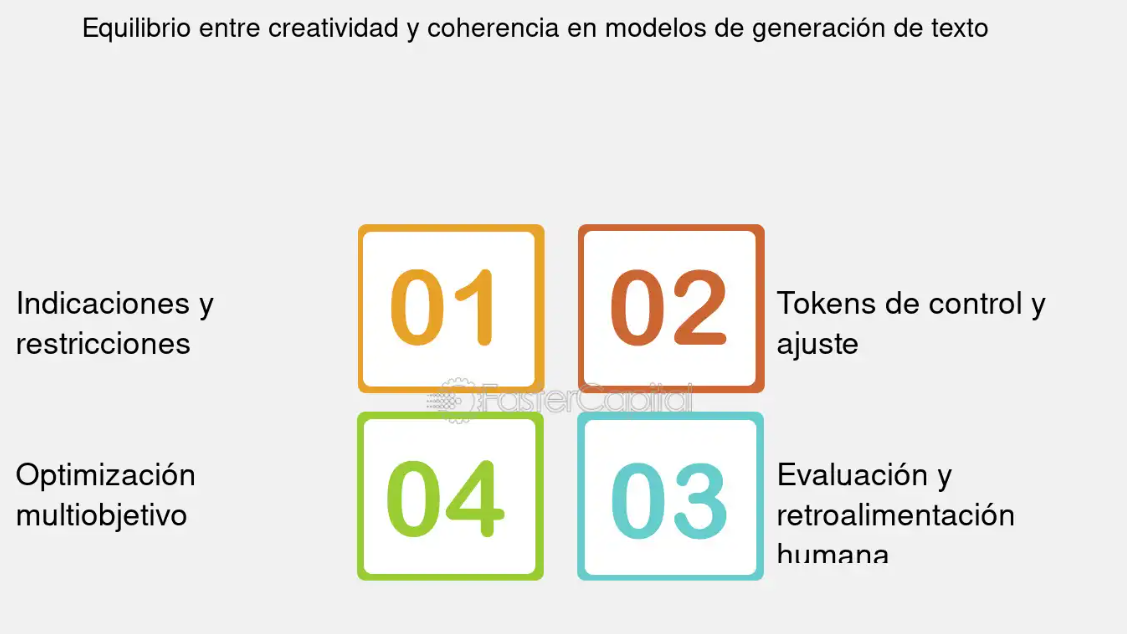
\includegraphics[width=.6\textwidth]{generacionCreativa.PNG}
    \label{fig:my_label}
\end{figure}

\subsection{ventajas}
\begin{itemize}
    \item Mejora la accesibilidad y facilita la redacción sin errores gramaticales.
    \item Puede ahorrar tiempo en la creación de contenido, desde artículos informativos hasta literatura creativa.
\end{itemize}

\subsection{Desventajas}
\begin{itemize}
    \item Existe el riesgo de creación de contenido repetitivo o con sesgo.
    \item Plantea preocupaciones éticas sobre la autoría y el plagio en la generación de textos automatizados.
\end{itemize}

\section{Conclusiones}

La inteligencia artificial está transformando rápidamente diversas áreas creativas y de entretenimiento, 
aportando herramientas poderosas tanto para usuarios como para profesionales. En los juegos, la IA permite desarrollar agentes 
inteligentes que responden dinámicamente, ofreciendo experiencias de juego más personalizadas y desafiantes. En el arte, las GAN y
otras tecnologías creativas impulsan nuevas formas de expresión, generando obras visuales que cuestionan los límites entre la creación humana
y la artificial. En la escritura, modelos de lenguaje avanzados facilitan la corrección de texto y la generación automática de contenido, 
democratizando la escritura y ampliando sus aplicaciones.
No obstante, la aplicación de la IA en estas áreas plantea desafíos importantes. En los videojuegos, existe el riesgo de que agentes 
excesivamente complejos afecten la experiencia de juego. En el arte, la generación automática puede restar valor a la labor humana y 
plantear cuestiones éticas sobre la originalidad y apropiación cultural. En la escritura, los modelos de generación de texto pueden 
producir contenido sesgado o éticamente cuestionable, lo cual exige regulaciones claras y un uso responsable.

\clearpage

\section{Bibliografia}
\begin{itemize}
    \item \href{https://www.iic.uam.es/innovacion/alphazero-y-el-go/}{Instituto de ingeniería del conocimiento}.
    \item \href{https://theblackboxlab.com/2024/02/23/deepmind/}{The blackBoxLab}.
    \item \href{https://www.linkedin.com/pulse/creatividad-artificial-est%C3%A1-la-ia-redefiniendo-el-concepto-e0djc/}{Sube Consultores}.
    \item \href{https://www.technologyreview.es/s/16532/que-es-la-inteligencia-artificial}{MIT technology review}.
    \item \href{https://www.sciencedirect.com/science/article/pii/S1136103423000114}{ScienceDirect}.
    \item \href{chrome-extension://efaidnbmnnnibpcajpcglclefindmkaj/https://www.reue.org/wp-content/uploads/2024/07/184-195.pdf}{REUE | Artículo especial}.


\end{itemize}

\end{document}
